\chapter{State of Art}
In this chapter, I firstly discussed the current researches in the realm of home automation system, in order to achieve inspiration materials for my demonstration scenario. Also after studying the industrial smart home application cases listed in this thesis, I have concluded that present-day automation systems commonly require a well-defined communication interface among all the housing devices, system as well as information security is still strongly demanded, which in return proofs that my proposal is meaningful and promising.  

The second topic covered by this chapter is the study of security. In more details, I have studied security   technologies and mechanisms employed in OPC UA standards as well as Smart Card system and Android applications. With the acknowledgment of aforementioned studies, I have learned the potential threads to my application system as well as how to provide corresponding countermeasures. Moreover, in the last paragraph, I introduced  the general guild-line for the development of a secure embedded system, which enlightened me about how to design my demonstration system.
 
\section{Smart Home Research}
\subsection{Overview}
The smart home system, which is also described as automated home, integrated home system or intelligent building \cite{smart_home_concept}, has drawn more and more industry developers' and researchers' attention over the decades. Research groups from for instance Siemens, IBM, Cisco, Microsoft has already contributed in this domain \cite{smart_home_research}. A great number of Smart Home applications, network protocols as well as gateways have come into world and been applied to benefit their customers \cite{smart_home_for_gateway}.

With the development of Smart Home technology, nowadays' Smart Home not only is in charge of monitoring and controlling lighting and heating devices inside the building, but also capable of connecting almost every electronic housing devices, inhabitant's behavior predicting as well as making scheduler decisions. Functionalities provided by intelligent home are not just limited to turn device on and off, record and report senor data, but include self-adjusting the inner building environment and supporting various predefined patterns, such as energy saving pattern. Especially the concept of Smart Home for elderly \cite{smart_home_for_old}, which perfectly combines modern remote control and monitoring technologies with senior-friendly and patient-concerning housing techniques, is welcomed by the market. 

Three categories of Smart Home will be introduced in the following as best practice examples, they are Smart Home optimized for energy services , Smart Health Home and Agent-based Smart Home.
 
\subsection{Smart Home Optimized for Energy Services}
This type of Smart Home sets its main goal in the energy saving and monitoring domain, which helps householder to make wiser decisions under the energy crisis background. 

The key component in this Smart Home is decision-support tool \cite{smart_home_for_energy}, that applies a scheduling algorithm which offers house owner energy saving suggestions based on various variables such as distributed energy resources (DER), with the prospect of saving precious energy and resource.

\subsubsection{Decision Support Tool}

 \begin{figure}[!htbp]
	\centering
	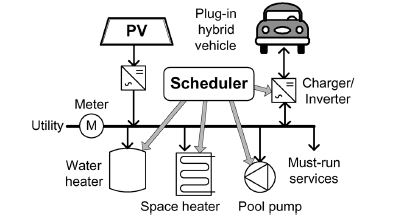
\includegraphics[width=1.0\textwidth]{scheduler.jpg}
		\caption{DER Scheduler in Smart Home optimized for energy\cite{smart_home_for_energy}}
	\label{fig:smart-home-scheduler}
\end{figure}

The decision support tool used in paper \cite{smart_home_for_energy} consists of two components, they are energy service model which describes the energy service request and distributed energy resource scheduling algorithm, as described in figure~\ref{fig:smart-home-scheduler}. To be more specifically, energy service model presents the demand of one particular energy resource. For instance the demand aimed at hot water means, the hourly consumption of heated water or the energy that is hourly needed by water heater.  According to paper \cite{smart_home_for_energy}, the heat content of water is also defined as "energy equivalent" and therefore the main goal of decision support tool is to increase "monetary benefit"  from every "energy equivalent" unit.

The DER scheduler algorithm, that helps householder to reduce the unnecessary consumption of energy, is in nature one mathematical optimization problem defined as following \cite{smart_home_for_energy}.
\begin{center}
 $ \sum_{t=1}^{T}\sum_{i=1}^{S}[\lambda_{ES,i}(t)\cdot {U_{ES,i}}(t,x)]-Cost$
\end{center}

The purpose of DER scheduler presented as \emph{x} is, to maximize that above introduced fitness function, where \emph{S} represents all number of services offered by Smart Home, \emph{T} stands for the whole simulation time, $\lambda_{ES,i}$ and $ U_{ES,i}$ describe the desired monetary benefit for "energy equivalent" and energy demand of the \emph{i}th service respectively. \emph{Cost} means the total electricity consumption. Also in paper \cite{smart_home_for_energy} the choice of DER algorithm is well discussed.


\subsection{Smart Health Home}
Another suitable application domain for Smart Home is the Smart Health Home, which describes the intelligent housing that takes care of patients at home or elder residents.

The charming feature of this Smart Home system is the combination of telemedical system with home automation technologies, which provides customized services such as, teleconsulting, telediagnosis, real time imaging as well as long distance medical education \cite{smart_home_for_health}. Smart Health Home will improve the living condition of householder and at the same time build a concerning system that takes care of residents' need. Nine best practice examples are provided and evaluated in paper \cite{smart_home_for_old}, they provide a guide-line for the design of Smart Health Home system and summarizes precious experience. 
 \begin{figure}[!htbp]
	\centering
	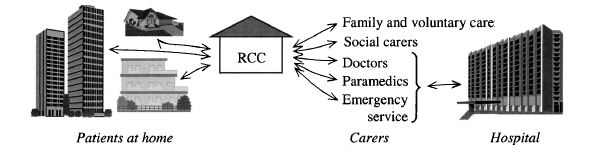
\includegraphics[width=1.0\textwidth]{rcc.jpg}
		\caption{Overview of Smart Health Home structure \cite{smart_home_for_health} (RCC: Remote Control Center)}
	\label{fig:rcc}
\end{figure}
\subsection{Agent-based Smart Home} \label{secAgent}
Agent-based Smart Home aims to build an intelligent home, which is based on machine learning, artificial intelligence technology and mobile computing. The core features of agent-based Smart Home are, prediction of householders' behaviors and making appropriate decisions. The achieved prediction can help residents to experience a more comfortable and convenient living condition. MavHome (Managing An Intelligent Versatile Home) builds the best demonstrating example \cite{smart_home_agent} . 

\subsubsection{MavHome architecture}
 \begin{figure}[!htbp]
	\centering
	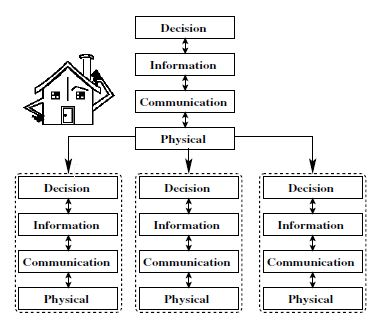
\includegraphics[width=0.8\textwidth]{smart-home-agent.jpg}
		\caption{MavHome agent architecture \cite{smart_home_agent}}
	\label{fig:smart-home-agent}
\end{figure}
As shown in figure~\ref{fig:smart-home-agent}, agents which are employed by MavHome consist of four different layers. From bottom to top:
\begin{itemize}
\item \emph{Physical layer}, where Smart Home system device hardwares are deployed. Moreover, underlaying agents can also act as physical layer for other high level agents.
\item \emph{Communication layer}, this layer provides communication service for agent by using functionalities offered by physical layer.
\item \emph{Information layer}, as higher layer of Smart Home system,  the responsibilities of this layers are gathering and maintaining information which is going to be required by decision layer.
\item \emph{Decision layer}, in this layer agents make decision as well as learn resident's preference. Moreover, with the help provided by learning algorithms, agent is also able to correct the unwanted system behavior and learn from bad decisions.
\end{itemize}
\subsubsection{Prediction algorithm}
Prediction algorithm is the core component of MavHome project. several strategies are presented on the first IEEE international conference on pervasive computes and communication, they are SHIP algorithm that is based on sequence matching, compression-based prediction algorithm ALZ and Task-based Markov model \cite{smart_home_agent}.

\subsection{Conclusion}
As described above, Smart Home is the representative application which is based on industrial automation, remote management and coordination system. Despite the decision making algorithms and application level components from above mentioned smart buildings are different from the other, but they all are integrated upon or connected with housing devices. The management and cooperation with those devices must take place under a secure system environment. None of householders are willing to be monitored by a strange third party using his own camera or to expose their daily life related information to the public. Therefore one common request for the design of such intelligent buildings is to ensure the system security.

Based on the fact, that home devices applied by Smart Home are manufactured by various vendors,  Smart Home designers also must take it into account, that how to realize the system interoperability. Considered those two requirements, the proposal of this thesis is proofed as practical and desired.

\section{OPC UA Application and Security Policy}

\subsection{OPC UA Applications}
OPC UA, as explained in former paragraphs,  is understood as a platform independent, well designed, security concerning, IEC standard compliant, promising industry standards set, which provides a service oriented architecture and is being widely applied in industry fields such as critical control system and industrial automation. Application cases are given in following paragraphs, each of them has different focuses. To be more specifically, the charming demonstrated characteristics of OPU UA applications are: strong security protection, real time data exchange as well as coordination and scalability. 

\subsubsection{OPC UA and ICS}
With the development of industrial automation technology, Industrial Control System (ICS) has became a hot topic, but most manufactures invested much more effort in designing automation as well as manufacturing process and neglected the communication security issues. As a consequence, cyber security of ICS is now drawing more and more attentions. OPC UA offers manufactures who are applying ICS system not only sophisticated object oriented modeling rules, which can be extremely helpful for developers to design domain specific model and manufacturing process, but also provides them a reliable and robust security model \cite{opc_ics}, that has various secure arrangements in each layer of software architecture.


\subsubsection{OPC UA and Smart Grid}
Smart Grid is now considered as the future of electricity energy industry and therefor how to achieve an intelligent electricity distribution as well as the coordination of behaviors between customs and suppliers becomes the most popular topic \cite{opc_grid}. Electricity industry is searching out for a standardized communication and connectivity technology to solve aforementioned issues.
OPC UA standards set that includes \emph{alarm and even} model, \emph{data access} model as well as  \emph{historical data access} model, is without doubt one the of best candidates. With the help of all aforementioned models, the secure real-time peer communication and coordination among stockholders are guaranteed.

\subsubsection{Nano OPC UA }
Apart from those enterprise level systems, OPC UA is also suitable for lower level field devices, such as field sensor and other resource limited facilities. Recently a German company Lemgo even designed a nano embedded OPC UA server \cite{opc_lemgo}, which provides the core OPC UA server service set. adopts TCP binary communication protocol and is implemented on a chip device.

\subsection{OPC UA Secure Policy}
At the beginning of OPC UA standards design phase, the OPC foundation has taken the construction of a secure and robust communication protocol as the center of their work and therefore developed an enhanced consistent security model which has clear and definite objectives in each layer of OPC UA software architecture. At the present day, OPC UA  offers secure messaging mechanisms by applying WS security with Simple Object Access Protocol (SOAP)  and alternatively SSL based Hypertext transfer Protocol Secure (Https) messaging \cite{opc_secure_1}. Besides secure messaging protocols,  authentication mechanisms based on username-password or X.509 certificates are also introduced, in order to perform mutual authentication among OPC UA applications from different logic levels and hardware devices.

OPC foundation introduces the term \emph{secure policies} \cite{O2} to describe the 
user authentication, user authorization, application authentication as well as message encryption mechanisms proposed by one OPC UA server profile. In this server profile, both secure related requirements and other server functionalities are described. One server is capable of maintaining several profiles in order to provides distinguishing services to different clients, who might have various security demands. Meanwhile one client can also accept a list of profiles, each of them is assigned by one server with particular security objective. 

\subsection{OPC UA Secure Consideration}
Along with core services set including data read and write operations, notification mechanism and etc, OPC UA server also provides \emph{discover service}  \cite{O4}, which provides OPC UA clients the mechanism to require server secure policy. Moreover a \emph{secure channel service} set \cite{O4} is also designed, which is applied to create and manage secure channel with acknowledgment such as key deviation algorithm and encryption algorithm, that are described by secure policy. 

Also OPC UA specifications provide guide lines for a secure system design \cite{O4}. They are:

\begin{itemize}
\item \emph{appropriate timeout}. Timeout mechanism is widely employed in systems that adopt client-server architecture. With reasonable configured timeout property, both client and server can avoid unnecessary resource consumption caused by long time waiting of response from the other, which could be the consequence of an unexpected physical device failure or denial of service attack, which is intentionally initiated by an adversary.
\item \emph{Message exchange rate control}. Rate control is considered as one of the most practical approach to prevent denial of service attack. Under rate control mechanism, each client has limited chance over a period to build communication channel, reconstruct this channel, require information from server or send data to server. Alternatively the OPC UA server can also ban or block a client for a period of time, who was recently trying to flood messages. 
\item \emph{random number generation}. The generation of random number is required by most encryption, authentication and authorization algorithms. Therefore a secure system must support and provide a robust random number generation function.
\item \emph{strict message processing}, which means the exchanged message between two communication partners must be compliant with predefined message format. Any ill-formed messages must be ignored, which in turn helps to avoid stack overflow attack and enhances system security
\item \emph{historical data management}, this strategy ensures the system traceability and records any behaviors taking place in system. The recorded data can be used for forensic research, when security related issue happens.
\end{itemize}
\subsection{Conclusion}
Above pictured OPC UA standards' features and characteristics proof the feasibility of applying OPC UA as communication protocol for Smart Home proposed in this thesis and the study of industrial application cases helps me to learn this point better.

\section{Smart Card Security}
Integrated circuit cards, ICCs for short, was firstly designed and patented in Germany \cite{smart_card_history}. Since then this credit sized, embedded with circuit chip card is being applied in more and more various industry domains as for instance information storage media, on-line access token, identification method, small amount payment mechanism and etc. With the development of smart card technologies, nowadays apart from traditional \emph{contact smart card}, \emph{contactless smart card} \cite{smart_card_contactless} has come into market. This \emph{contactless smart card} is able to communicate with card accepting device without direct physical connection. To be more precisely, it applies radio frequency to contact with CADs. Now matter what categories of smart card, the tamper resistant nature always contributes to make them to be the most popular secure token media.
\subsection{Smart Card in Access Control Management}\label{secSCAC}
The present-day concept of \emph{security} no longer just meant the secure of our homeland borders or the individual personal safety. In this information age, the word \emph{security} also refers to the confidentiality and integrity of users' personal data, the robustness of information system and so on. It is immediately related with our daily life. Especially when electronic devices, which can carry sensitive as well as precious information and could be vulnerable to malicious attackers, are playing irreplaceable roles in our society. 

Smart card, as explained in section \emph{fundamental technologies}, is believed as one of the best secure mechanism for access control and user identification. 

Traditionally there are three ways to identity a person \cite{handbuch}:
\begin{itemize}
\item \emph{1 knowledge about a secret}, the secret is normally a password that negotiated earlier between two identification peers.
\item \emph{2 possession of an object}, this object could be anything that is predefined. One example could be the key that can open a particular door.
\item \emph{3 biometrics identification}. First two points have their own limitations, because third part could steal the object, that is used for identification, or copy user's password. Moreover it also can happen, that a password is too complex to remember or identification object is hard to carry with. Compared with them, biometrics identification depends on however the human body characteristics, such as fingerprint, signature and retina recognition.
\end{itemize}
Based on the above described facts, smart card is the best candidate for user identification and access control. Because when anyone wants to perform identification using smart card, he must possess the card (possession of an object satisfied), input PIN to unlock the card (knowledge about a secret). At the same time, complex passwords for the purpose of peer authentication and authorization can be stored on the smart card, which helps card holder to release the burden of remembering them. Also on a chip name card, which is usually carried by a card-holder in order to access a secured room or building, there usually exists a signature signed by the card-holder or his photo, that could be use to perform biometrics identification. 

Nowadays with the help of standards such as \emph{remote application management} protocol, which is introduced in \emph{fundamental technologies} section~\ref{secGP}, smart card is also capable of performing on-line identification based on either certificate or TLS protocol.

\subsubsection{Personal Identification Number}
Whenever an user intends to use one smart card, he must input a \emph{personal Identification Number}, which is also referred as \emph{Card Holder Verification}. PIN consists usually of four decimal number from 0 to 9 and tolerates at most 3 times wrong PIN input before a successful verification. PIN is stored in elementary files  \cite{smart_card_access} on smart card in order to be kept from unauthorized modification. After 3 times wrong PIN input, a smart card will be locked until the \emph{unlock PIN} operation is successfully carried out. Moreover if \emph{unlock PIN} operation also fails three times in a roll, the PIN will never be unblocked \cite{smart_card_access}.

\subsection{Smart Card Key Management Mechanism} \label{labelKeyManagement}

 \begin{figure}[!htb]
	\centering
	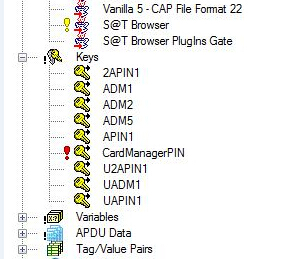
\includegraphics[width=0.45\textwidth]{smart-card-key.jpg}
		\caption{keys presented in Smart Card Description Language from \emph{Morpho}}
	\label{fig:smart-card-key}
\end{figure}

The above introduce PIN is not the only key that is stored on smart card. In order to perform message encryption as well as decryption, peer authentication and etc. smart card must keep various keys in storage. As shown in figure~\ref{fig:smart-card-key}, in one \emph{Morpho} smart card product, a list of keys and key sets are used, for example, Card Manager PIN and Administrative keys (\emph{ADM1, ADM2, ADM5}).

Moreover key data in smart card not only simply records the actual key value but also provides information such as key version number and the usage of key as shown in Table~\ref{table:smart-card-key}. Likely the usage of a key also needs more information than just input one key value as shown in figure~\ref{fig:smart-card-key-use}.

 \begin{figure}[!htb]
	\centering
	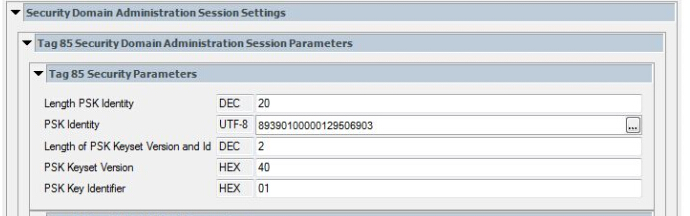
\includegraphics[width=0.85\textwidth]{smart-card-key-use.jpg}
		\caption{the PSK key used to configure administration session}
	\label{fig:smart-card-key-use}
\end{figure}

\begin{table}[!htb]
\caption{key data stored in smart card\cite{handbook}}
\begin{tabular}{lllll}
\hline\hline
Data object & Remarks\\[0.5ex]
Key number & unique key reference number\\
Version number & version number used for key derivation\\
Intended usage & for which purpose this key is introduced\\
Blocked & used to block a key\\
Retry counter & wrong key input counter\\
Maximum retry count & key will be blocked if retry counter reaches this value\\
Key size & the size of key\\
Key & Key value\\
\hline
\end{tabular}
\label{table:smart-card-key}
\end{table}

Since different keys play distinguishing roles in various system tasks and smart card must handle a huge number of keys, \emph{key management} mechanism shows its importance. The core responsibilities of smart card key management system are listed as following \cite{handbook}:
\begin{itemize}
\item \emph{key generation.} Key generation is the initial step of key life cycles and uses usually physical random numbers as initial data, in order to generate secure and unique keys. 
\item \emph{key update.} This process keeps one key from being used for a long period. Because long time service of one key could lead to the compromise of system security.
\item \emph{key revocation.} When one key turns out to be compromised, key management system must destruct that key.
\item \emph{key storage.} Apparently a competent key management system must know how to safely store its secrets.
\end{itemize}
\subsubsection{Key Generation}
\paragraph{Derived Key}
Since smart card can be easily exposed and analyzed by anyone who holds or steals the card, in order to minimize the risk of key compromising, none master keys are present in smart card. As a consequence, keys used in smart card are derived from unique card number, which is given during the card production process, with the help of triple DES and AES cryptographic algorithms \cite{handbook}.
\paragraph{Dynamic Key}
Dynamic key is normally applied to protect communication between peers and therefore it is also known as the session key or temporary key. The generation of dynamic keys begins with the generation of a random number that is proposed by one communication partner or unique data which is able to specify one particular session. There is a number of dynamic key generation approaches and I will take \emph{ANSI X 9.17} standard as an example \cite{handbook}. 
\begin{center}
$Key_{i+1} = e(Key_{gen},e(Key_{gen},(T_{i} XOR Key_{i})))$
\end{center}
The function described above is one-way process and can not be reserved. To be more specifically, $T_{i}$ and  $Key_{gen}$ are the time as well as session independent initialization input parameter and Key generation key respectively. The newly generated  key $key_{i}$ can not only be used for encryption but also to generate other new keys.
\subsection{Threatens and Countermeasures}
In this section, potential smart card vulnerabilities, threatens aimed at chip card as well as countermeasures will be discussed. But before we begin the analysis of smart card threatens, the trust environment of smart card based system should be explained. Following five parties are involved \cite{smart_card_attack1}.
\begin{itemize}
\item \emph{Cardholder.} In other word, the owner of smart card, who daily applies smart card for different purposes in various systems. For instance, using SIM card in cell phone to make phone call or using smart card digital wallet to perform smart amount payment like paying the parking fee.
\item \emph{Terminal.} Terminal is the card accepting device that communicates with smart card through smart card I/O.
\item \emph{Card Manufacturer.} As the name indicates, card manufacturer is the one who manufactures  the card.
\item \emph{Card Issuer.} Card Issuer is the party that designs the card OS and initializes the smart card. For example, if we are taking about a cell phone smart card, then card issuer will be the cell phone service provider. When it comes to employees' ID cards which are applied as access control tool for a company. Then in this situation, the card issuer is the employer.
\item \emph{Software manufacturer.} This party is the one who designs applications that run on smart card.
\end{itemize}
\subsubsection{Smart card Threatens and vulnerabilities}
Since threat modeling for smart card could be extreme complex and also the classification of smart card is various. In this paragraph four representative threaten categories are presented. They are,
\begin{itemize}
\item Logical attacks. Whenever we develop a software, there could exist a bug/bugs. And logical attacks just refer to the attacks that make use of bugs in software implementation \cite{smart_card_attack2}. Two examples are given as follow:
\begin{itemize}
\item \emph{Hidden Commands}. This kind of attack attempts to abuse some commands from \emph{initialization phase} of smart card life cycle, to modify or retrieve sensitive data from smart card in poorly designed smart card system. The abused command should have been inactive but not in above mentioned vulnerable system \cite{smart_card_attack2}.
\item \emph{Malicious Applets}. Ill-designed smart card software, that attempts to break smart card system and steal information.
\end{itemize}
\item Physical attacks. This type of attack aims to reverse engineer the data and functions that are contained on smart card. Normally expensive and modern lab equipments are required \cite{smart_card_attack2}. Also physical attack is known as \emph{invasive attack} \cite{smart_card_attack3}. Three kinds of physical attacks are introduced as following :
\begin{itemize} 
\item \emph{Micro-probe station}. Using Micro-probes, adversaries try to construct electrical connection with smart card chip, in order to observer communication between process and memory. With the observed information, attacker is capable of capture sensitive data such as key information and etc \cite{smart_card_attack3}.
\item \emph{Focused Ion Beam}. Also it is possible to transmit intentionally generated signals to smart card processor using focused ion beam. As a consequence, it is possible for attacker to reveal data from smart card \cite{smart_card_attack3}.
\item \emph{Chemical Solvents, Etching and Staining Materials}. Using aforementioned chemical materials, attacker can observe etching speed difference from some ROM memories and with a step further analyze \emph{0} and \emph{1} in those memories \cite{smart_card_attack2}.
\end{itemize}
 \begin{figure}[!htbp]
	\centering
	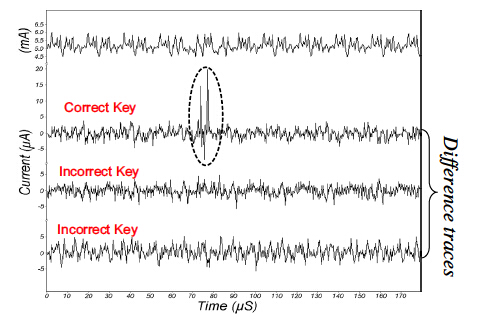
\includegraphics[width=0.8\textwidth]{pda-attack.jpg}
		\caption{Differential Power Attack on a DES implementation \cite{embedded_secure}}
	\label{fig:pad-attack}
\end{figure}
\item Non-invasive attacks. This kind of attack makes use of smart card runtime environments such as difference in power consumption, processor voltage, clock frequency and etc. to analyze smart card behaviors. For example,
\begin{itemize}
\item Power consumption attacks. The execution of smart card operations relays on power provided by terminal.  When attacker is able to observe smart card power consumption, which is used by card performing cryptographic algorithms, he may retrieve related keys by applying \emph{Differential Power attack} or \emph{Single Power attack} \cite{smart_card_attack3}. Figure~\ref{fig:pad-attack} pictures a differential power attack analysis on a DES implementation.
\item Timing attack on RSA. The computing duration of RSA algorithm depends also on the input key. Therefore there is an opportunity for attacker using observed time gap in key computation to get secret key information \cite{smart_card_history}
\end{itemize}
\item Other Attacks\cite{smart_card_attack5}.
\begin{itemize}
\item Denial of service. This kind of attack aims at impacting smart card performance and consuming smart card system recourses to harm the availability of smart card service .
\item Eavesdropping. Through eavesdropping exchanged information is catapulted and analyzed.
\item Cover transaction. Fake session or session hijacking. Those approaches try to forge a communication session between smart card and the other connection peer, in order to gain information, which is related with peer authentication, authorization and messaging.
\end{itemize}
\end{itemize}

\subsubsection{Countermeasures} \label{secSMD}
\paragraph{Logical Attacks Countermeasure}
In oder to prevent this category of attacks, the number of bugs in smart card application should be minimized. Software and card manufacturers can apply \emph{structure design} by dividing application into small units which are easy to be tested and understood. Alternatively various company related in smart card industry should work together to propose standardized interfaces and protocols to regulate the application development process \cite{smart_card_attack2}.
\paragraph{Physical Attacks Countermeasure}
Smart card manufacturers have already realized the potential  invasive attacks and are enhancing the physical security of smart card by offering:
\begin{itemize}
\item Reducing chip size. Now the size of smart card internal components can reach 150 nm, which makes it significantly hard for attacker to perform physical attack \cite{smart_card_attack3}.
\item Metalization layers, which prevent smart card from atmospheric effects \cite{smart_card_attack3}.
\item Multi-layered chips. Smart card manufactures are now able to build chip card consisting of multi-layers. Vulnerable components, for instance ROM memory, are deployed in the lowest layer and protected from physical analysis \cite{smart_card_attack3}. 
\item Sensors.  Smart card is protected by sensors covered with resin and those sensors will disable smart card whenever they detect physical attacks \cite{smart_card_attack}.
\end{itemize}
\paragraph{Non-invasive Attacks Countermeasure}
Countermeasures against above described non-invasive attack are:
\begin{itemize}
\item Against Timing Attacks by computing \emph{superfluous calculations}, in this way adversaries are not able  to get correct timing gap anymore \cite{smart_card_attack3} .
\item Against Power Consumption Attacks by applying digital noise. Alternatively chips manufacturers can reduce the electromagnetic emissions to make power consumption analysis  harder\cite{smart_card_attack3}.
\end{itemize}
\paragraph{Other Attacks Countermeasure}
Other attacks are normal computer security issues and can be avoided by for instance applying message encryption mechanism, building communication session based on secure channel, introducing message transmitting rate control policies and defining appropriate timeout counts.
\subsection{Smart Card Secure Applications}
As given above, smart card is considered as a secure data storage media and a superior tool to protect information system security. People also describes smart card as the \emph{magic bullet}, that can solve computer security issues, such as access control management, peer identification and so on. Understandably, therefore more and more smart cards are applied in secure applications and products. For instance:
\begin{itemize}
\item In Payment System. Recently the concept of electronic purses and electronic payment systems becomes more and more popular. Not only because this newly proposed mean of payment can play a supporting role for traditional payment methods such as credit card, but also because with the integration of smart card, electronic purses are able to offer flexible, reliable and secure small amount payment  services \cite{handbook}.
\item For Peer Identification. Based on the knowledge from section~\ref{secSCAC}, Smart card holder is  capable of performing two factor authentication \cite{smart_card_history}, which requires that at least two of three listed conditions are satisfied. Therefore smart card are suitable for the domain of personal identification. Since December 1999, Finland has begun to use electronic personal ID cards to replace traditional passports \cite{handbook}. 
\end{itemize}
\subsection{Conclusion}
In conclusion, the above discussed security features of smart cards, such as sophisticated key management system and counter measures against potential threads, proof the feasibility and reliability of my proposal, that is applying smart card for secure credential management and adding additional protection for the system which adapts smart card. Moreover with the help of industrial standardized protocols which are introduced in section~\ref{secGP}, card holder can enjoy a secure remote management service and trust the electronic devices which are integrated with smart cards, let those facilities administer his properties.  

\section{Secure Android Design}
With the development of smart phone market, more and more subscribers are using this new generation of cell phones with their smart cards. Accordingly an increasing number of attacks aimed at smart phone platforms is reported. 

 \begin{figure}[!htb]
	\centering
	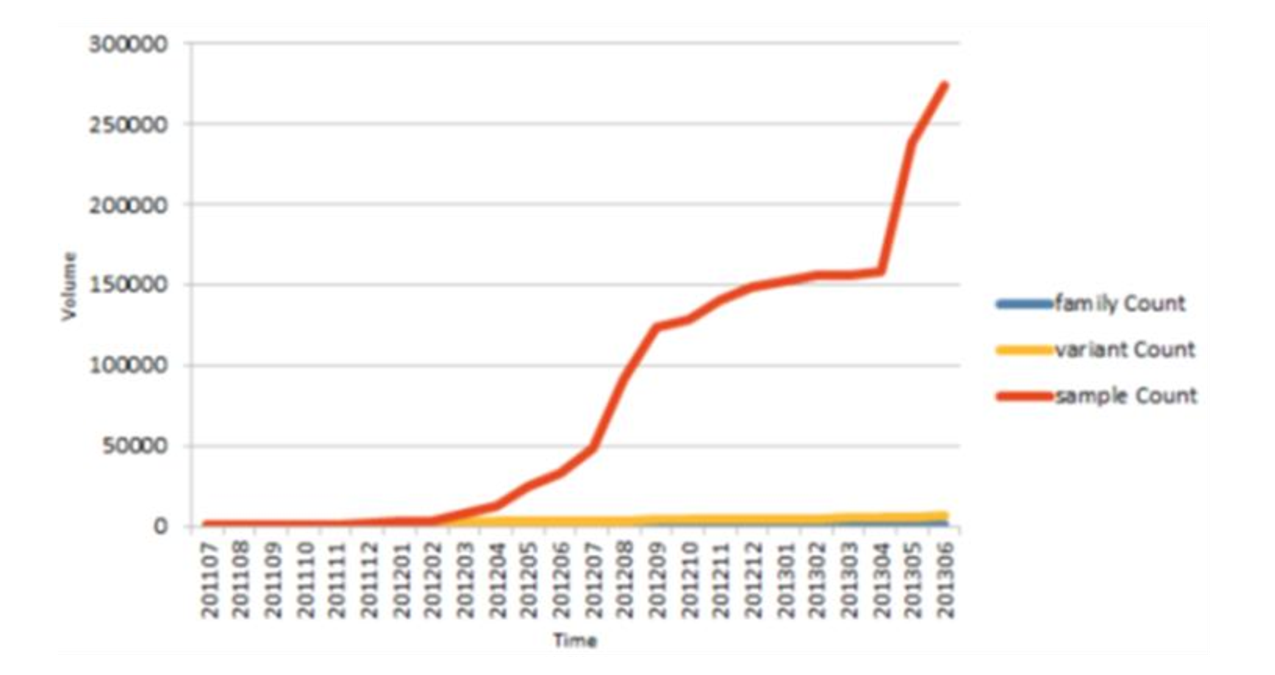
\includegraphics[width=1.0\textwidth]{malware1.pdf}
		\caption{Android Malware Growth \cite{malware}}
	\label{fig:android-malware}
\end{figure}

Figure~\ref{fig:android-malware} shows a dramatic increasing amount of Malwares that are targeted at Android from report \cite{malware}. Especially when taken it into account that present-day smart phones are also in charge of sensitive users' information such as recent visited location as well as contacts list.  And based on a study of Android applications, researchers have found that over 20\% applications could have access to user personal data \cite{android_secure_design}. Consequently there exists a pressing requirement for Android application developers to design an Android software with strong security protection. 

\subsection{Android Security Mechanism}
Even though a huge number of third party applications exist on Android market and they could be potential Malwares, but Android platform is not vulnerable and it provides secure as well as robust security mechanisms to protect its customers. Following listed three methods are the most outstanding and efficient approaches.
\begin{itemize}
\item \emph{Application Isolation.} Each Android application has its own Linux process and each of this process possesses an isolated virtual machine. In this way, application data is separated and protected from the other \cite{android_secure_language}. 
\item \emph{Access Permissions.} Permissions are given during the applications' installation time. As illustrated in figure~\ref{fig:android-permission}, Android permission system restricts the access right to user's private data, to other Android applications , to smart phone hardwares and to Android OS. 
\begin{figure}[!htb]
	\centering
	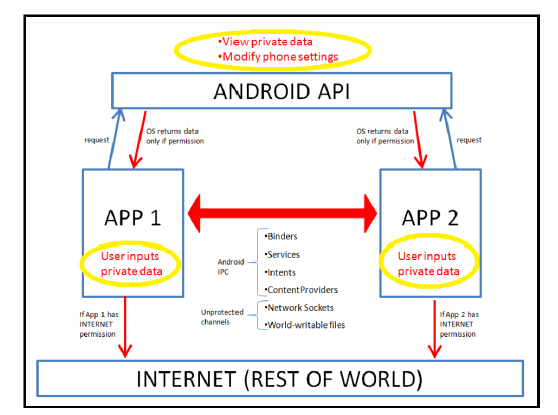
\includegraphics[width=0.9\textwidth]{android-permission.jpg}
		\caption{Detailed Android Permission Model \cite{android_secure_design}}
	\label{fig:android-permission}
\end{figure}
\item \emph{Authorized Signatures.} Applications are signed with certificates. The corresponding private keys are protected only by the application developer. Every time when one application claims his identity, his signatures will be checked, in order to prevent the potential masquerade attacks \cite{android_secure_language}.
\end{itemize}

\subsection{Security Design Guide-Lines}
With the acknowledgment from previous paragraphs, it can be concluded that Android system is designed with consideration of security, especially in the domain of access control and permission management. But still ill-developed application is vulnerable. For instance, when an application carelessly sends an intent introduced in section~\ref{secIntent}, which has none explicit target. This implicit intent can be intercepted by a Malware. As a result, this malicious application may manage to access the sensitive data of victim application and perform attacks such as \emph{activity hijacking} and \emph{service hijacking} \cite{android_secure_inter}.

Therefore it it necessary for application developers to apply protection techniques  in oder to protect their application from attackers and revers engineering. In the following, three secure Android design guide lines are summarized.

\subsubsection{Application Components Secure}
In order to restrict the number of applications, which have access rights to the Android application components described in subsection~\ref{secAppComponents}. Android application designer  should explicitly claim the access control policies in \emph{AndroidManifest.xml} from their project. In extreme case that none applications are expected to invoke the secured component, following rule should be added in \emph{AndroidManifest.xml} \cite{android_secure_cook}.
\begin{Verbatim}[fontsize=\relsize{-1},frame=lines,framesep=4mm, label=\fbox{\small\emph{Component Securing}}]
<[component name] android:exported='false'>
</[component name]>
\end{Verbatim} 

\begin{figure}[!htb]
	\centering
	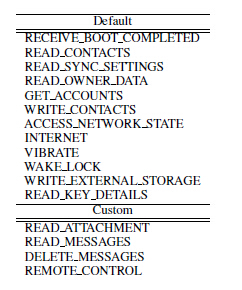
\includegraphics[width=0.4\textwidth]{android-permission2.jpg}
		\caption{Permission Required by Application \emph{k9mail} \cite{android_secure_design}}
	\label{fig:android-permission2}
\end{figure}
\subsubsection{Custom Permissions for Access Control}

As pictured in figure~\ref{fig:android-permission2}, Android OS provides a list of default permissions, which service a generic access control management, including such as  phone  holder data reading and writing, Internet access right and etc. But when it comes to the case of sharing data between different applications, a more sophisticated and robust custom permission is desired. To be more specifically, following xml snippets, which declare customized permission rules, should be added to the protected components in project's \emph{AndroidManifest.xml} \cite{android_secure_cook}.

\begin{Verbatim}[fontsize=\relsize{-1},frame=lines,framesep=4mm, label=\fbox{\small\emph{Custom Permission Snippet}}]
<permission android:name='android.permission.CUSTOM_PERMISSION'
	android:protectionLevel ='dangerous'
	android:description = 'Custom Permission Snippet'
	android:label = '@string/custom_permission_label''>
\end{Verbatim} 
Moreover four categories of protection level are supported \cite{android_secure_cook}:
\begin{itemize}
\item \emph{normal.} This the lowest level of permission and usually be applied for nondangerous permissions. 
\item \emph{dangerous.}  In this kind of permission, there exist the risks that authorized application would be able to access user credential information and sensitive data.
\item \emph{signature.} Signature permission means that applications which are signed with the same certificate can access each other.
\item \emph{signatureOrSystem.} In addition to \emph{signature} level, this level of permission will be also automatically granted to the application that is part of system image.
\end{itemize}
\subsubsection{Securing Content Provider}
Last secure approach that I want to present is the content provider path  secure mechanism. Since content provider handles mostly the exchanged data between applications, therefor it frequently becomes the first victim of a system attack. Application developer must ensure the security of content provider, especially the content provider path, which is in nature an uniform recourse identifiers that is related  to sensitive information such as datasets \cite{android_secure_cook}. Content provide path may look like \emph{content://com.provider.android/account/balance}.

It is highly recommended that application developer explicitly defines the permission rules at path level, one demonstration example is given as following \cite{android_secure_cook}, 
\begin{Verbatim}[fontsize=\relsize{-1},frame=lines,framesep=4mm, label=\fbox{\small\emph{Content Path Securing}}]
<provider ...>
<grant-uri-permission android:path = 'path_name'>
</provider>
\end{Verbatim} 
\subsection{Conclusion}
In conclusion Android is  a secure platform with sophisticated access control mechanisms and other security polices. But still Android application developers should apply security techniques to protect their project from malicious and ill-formed applications. Moreover I developed my Android Application \emph{Smart Home App} following the above presented Android secure design guide lines. The concrete design and implementation details will be presented in following other chapters. 

\section{Embedded System Secure Design}
\subsection{Overview}
In this last section, a generic guide for the embedded system secure design is introduced. As already in previous sections described, low level components that build the embedded system compared with traditional  computer software have additional security requirement. For instance, low end devices are normally dependent on battery as electricity supplement and have limited computing capacities. Those two constrains must be taken into account during the design phase of a secure embedded system.
\subsection{Embedded System Secure Requirements}
The \emph{Trinity of Trouble} \cite{embedded_secure} three factors, namely \emph{complexity},\emph{extensibility} and \emph{connectivity} contribute together to make the embedded system more vulnerable and make the  system secure requirements complexer.
In the following a brief discussion about embedded system security requirements and corresponding solutions are presented \cite{embedded_secure}.
\begin{itemize}
\item \emph{User Authentication}. Before the embedded system performs any functionalities, the identity of system user must be confirmed. Alternatively the user also has the need to verity the embedded system's identity. The expected mutual authentication can be realized by applying secure protocol such as \emph{TLS 1.2} or using digital certificates and signatures.
\item \emph{Content Security}. The security of exchanged message also plays an import roll in a secure embedded system. Message integrity and confidentiality must be ensured. Popular solutions are to apply cryptographic algorithms such as symmetric ciphers, asymmetric ciphers and hash algorithms to protect system content from illegitimate modification and eavesdropping.
\item \emph{Secure Network Connection}. Most devices nowadays have the access to the Internet. As a consequence, secure  network connection belongs also to the security domain in embedded system. In order  to provide a secure network environment, system developer should apply secure communication protocols such as SSL or create secure VPN connection \cite{embedded_secure}.
\item \emph{Secure Storage}. System data must be protected from unauthorized modification and stealing by malicious entities. Therefore tamper resistance hardware should be applied.
\item \emph{Availability}. At last the service availability must be guaranteed by apply anti-Dos attack mechanisms, which are already introduced in this thesis.
\end{itemize}
\subsection{Software Security during Software Design Life Cycle}
\begin{figure}[!htb]
	\centering
	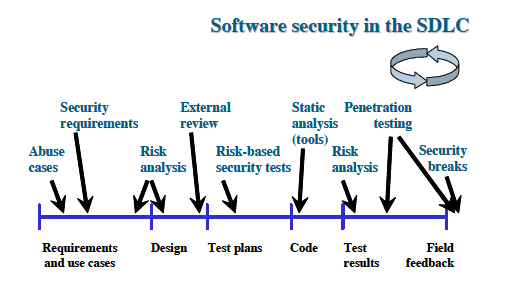
\includegraphics[width=0.95\textwidth]{sdlc.jpg}
		\caption{Software Security Consideration in Software  Design Life  Cycle \cite{embedded_secure}}
	\label{fig:sdlc}
\end{figure}
With the acknowledgment of system security requirements as well as corresponding solutions, embedded system designer should concern potential security threads as well as system imperfections in each applicaiton design phase and perform corresponding secure analysis as well as run secure-related tests, as shown in figure~\ref{fig:sdlc}.

\subsection{Secure Architectures}
In oder to keep an embedded system from malicious parities' attacks, especially when present-day system is normally exposed in a ubiquitous networking and pervasive computing environment \cite{embedded_secure}. System developer should design a robust and secure system architecture with the security consideration from architectural micro level to macro level. Figure~\ref{fig:design-space} pictures the choice of architectural design space.\footnote{ASIC:application-specific instruction set processor. EP: embedded general-purpose process. SPx: special purpose extensions. GPx:general purpose extensions. HWaccel: hardware accelerators. GOP: co-processor}
\begin{figure}[htb]
	\centering
	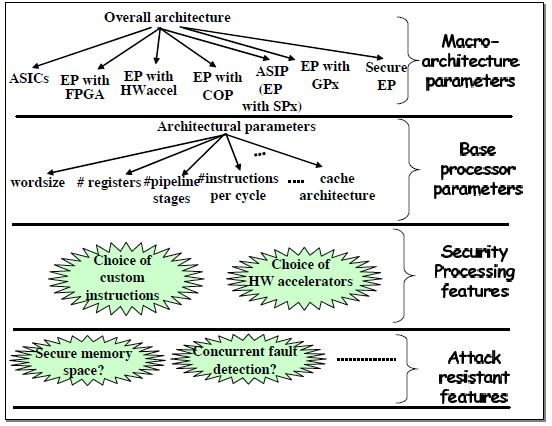
\includegraphics[width=0.9\textwidth]{design-space.jpg}
		\caption{Architectural Design for a Secure Information Processing \cite{embedded_secure}}
	\label{fig:design-space}
\end{figure}

When the hardware architecture characteristics of an embedded system are confirmed. Following two secure aspect as shown in last two rows in figure~\ref{fig:design-space} should be considered
\begin{itemize}
\item \emph{Security Processing Features.} Various fundamental secure protocols and algorithms could be selected by system designer. But some of them may offer the same security services. Therefore in this layer, the choice of cryptographic algorithms should be made with consideration from hardware and software specific aspect. For instance, the full implementation of SSL protocol for a simple low end PAD device might not be a wise decision \cite{embedded_secure}.
\item \emph{Attack Resistant Features.} When general security mechanisms used to ensure content confidentiality, data integrity and peer authentication are provided by a embedded system, attempts to prevent other kinds of security attacks such as denial of service attack also should be made.
\end{itemize}

\section{Conclusion}
In this chapter, I presented industrial application cases in the realm of home automation, OPC UA specifications and smart card products. Moreover I emphasized the importance and significance of security in those applications. Also, I discussed the secure mechanisms employed by smart card, the OPC UA secure policies, secure Android design as well secure embedded system development. The aforementioned technologies and secure approaches are applied in my demonstration system and will be presented in following chapters.

In next chapter, I am going to present the concept of my Smart Home system and associating components.